%%%%%%%%%%%%%%%%%%%%%%%%%%%%%%%%%%%%%%%%%
% Simple Sectioned Essay Template
% LaTeX Template
%
% This template has been downloaded from:
% http://www.latextemplates.com
%
% Note:
% The \lipsum[#] commands throughout this template generate dummy text
% to fill the template out. These commands should all be removed when 
% writing essay content.
%
%%%%%%%%%%%%%%%%%%%%%%%%%%%%%%%%%%%%%%%%%

%----------------------------------------------------------------------------------------
%	PACKAGES AND OTHER DOCUMENT CONFIGURATIONS
%----------------------------------------------------------------------------------------

\documentclass[12pt]{article} % Default font size is 12pt, it can be changed here

\usepackage[italian]{babel}
\usepackage[utf8]{inputenc}
\usepackage{geometry} % Required to change the page size to A4
\usepackage{graphicx} % Required for including pictures
\usepackage{float} % Allows putting an [H] in \begin{figure} to specify the exact location of the figure
\usepackage{wrapfig} % Allows in-line images such as the example fish picture
\usepackage[dvipsnames]{xcolor}
\usepackage{acronym}
\usepackage{lipsum} % Used for inserting dummy 'Lorem ipsum' text into the template
\usepackage{listings}

\geometry{a4paper} % Set the page size to be A4 as opposed to the default US Letter

\linespread{1.2} % Line spacing

%\setlength\parindent{0pt} % Uncomment to remove all indentation from paragraphs

\graphicspath{{img/}} % Specifies the directory where pictures are stored

\definecolor{back}{rgb}{1,0.93,0.76} 
\lstset{ %
	backgroundcolor=\color{back},  % choose the background color; you must add \usepackage{color} or \usepackage{xcolor}; should come as last argument
	basicstyle=\tiny,        	% the size of the fonts that are used for the code
	breakatwhitespace=false,        % sets if automatic breaks should only happen at whitespace
	breaklines=true,                % sets automatic line breaking
	captionpos=b,                   % sets the caption-position to bottom
	commentstyle=\color{gray},   % comment style
	frame=single,	                % adds a frame around the code
	keepspaces=true,                % keeps spaces in text, useful for keeping indentation of code (possibly needs columns=flexible)
	keywordstyle=\color{blue},      % keyword style
	language=Python,               	% the language of the code
	numbers=none,                   % where to put the line-numbers; possible values are (none, left, right)
	numbersep=5pt,                  % how far the line-numbers are from the code
	numberstyle=\tiny\color{black}, % the style that is used for the line-numbers
	rulecolor=\color{black},        % if not set, the frame-color may be changed on line-breaks within not-black text (e.g. comments (green here))
	showspaces=false,               % show spaces everywhere adding particular underscores; it overrides 'showstringspaces'
	showstringspaces=false,         % underline spaces within strings only
	showtabs=false,                 % show tabs within strings adding particular underscores
	stepnumber=1,                   % the step between two line-numbers. If it's 1, each line will be numbered
	stringstyle=\color{OrangeRed},    % string literal style
	tabsize=2                   	% sets default tabsize to 2 spaces
}

\acrodef{PCA}{\emph{Principal Component Analysis}}

\begin{document}

%----------------------------------------------------------------------------------------
%	TITLE PAGE
%----------------------------------------------------------------------------------------

\begin{titlepage}

\newcommand{\HRule}{\rule{\linewidth}{0.5mm}} % Defines a new command for the horizontal lines, change thickness here

\center % Center everything on the page

\textsc{\LARGE Università degli studi di Firenze}\\[1.5cm] % Name of your university/college
\textsc{\Large Corso di Laurea Magistrale in Informatica}\\[0.5cm] % Major heading such as course name
\textsc{\large Multivariate Analysis and Statistical Learning}\\[0.5cm] % Minor heading such as course title

\HRule \\[0.4cm]
{ \huge \bfseries Principal Component Analysis: dalla teoria alla pratica}\\[0.4cm] % Title of your document
\HRule \\[1.5cm]

\begin{minipage}{0.4\textwidth}
\begin{flushleft} \large
\emph{Autore:}\\
Marco \textsc{Buracchi} % Your name
\end{flushleft}
\end{minipage}
~
\begin{minipage}{0.4\textwidth}
\begin{flushright} \large
\emph{Docente:} \\
Prof.ssa Anna \textsc{Gottard} % Supervisor's Name
\end{flushright}
\end{minipage}\\[4cm]

{\large \today}\\[3cm] % Date, change the \today to a set date if you want to be precise

%\includegraphics{Logo}\\[1cm] % Include a department/university logo - this will require the graphicx package

\vfill % Fill the rest of the page with whitespace

\end{titlepage}

%----------------------------------------------------------------------------------------
%	TABLE OF CONTENTS
%----------------------------------------------------------------------------------------

\tableofcontents % Include a table of contents

\newpage % Begins the essay on a new page instead of on the same page as the table of contents 

%----------------------------------------------------------------------------------------
%	TESTO
%----------------------------------------------------------------------------------------

\section{Principal Component Analysis} % Major section

	\lipsum[1]
	
	\subsection{Subsection 1} % Sub-section

		\lipsum[1] % Dummy text

	\subsection{Subsection 2} % Sub-section

		\lipsum[2] % Dummy text

\section{Implementazione Python} % Major section

	Passiamo adesso all'implementazione di un piccolo esempio di \ac{PCA} sul dataset \emph{IRIS}. Per questa realizzazione è stato scelto il linguaggio \emph{Python} con la relativa libreria \emph{pandas}.

	\subsection{PANDAS} % Sub-section

		pandas è una libreria Python open-source, ad alte prestazioni e con licenza BSD che fornisce strutture dati e strumenti per l'analisi facili da usare.
		\begin{wrapfigure}{l}{0.3\textwidth} % Inline image example
			\begin{center}
				
\includegraphics[width=0.28\textwidth]{numFocus.png}
			\end{center}
		\end{wrapfigure}
		\`{E} un progetto sponsorizzato da NumFocus. Questo assicura lo sviluppo continuo e a livello mondiale e permette anche di aiutare gli sviluppatori con donazioni o citazioni.Permette di lavorare con dati organizzati in maniera \emph{relazionale} o \emph{etichettata} in maniera intuitiva. Le sue due strutture dati principali sono le serie (unidimensionali) e i dataframe (bidimensionali). Per il nostro esempio utilizzeremo questa seconda struttura.
		

	\subsection{Implementazione} % Sub-sub-section
	
		Come già detto, utilizzeremo il dataset IRIS che contiene 150 misurazioni di fiori iris di tre specie diverse. La figura \ref{fig:iris} schematizza le variabili del dataset che sono:
		\begin{itemize}
			\item Larghezza dei sepali in cm
			\item Lunghezza dei sepali in cm
			\item Larghezza dei petali in cm
			\item Lunghezza dei petali in cm
			\item Specie (setosa,versicolor,virginica)
		\end{itemize}
		\begin{figure}
			\begin{center}
				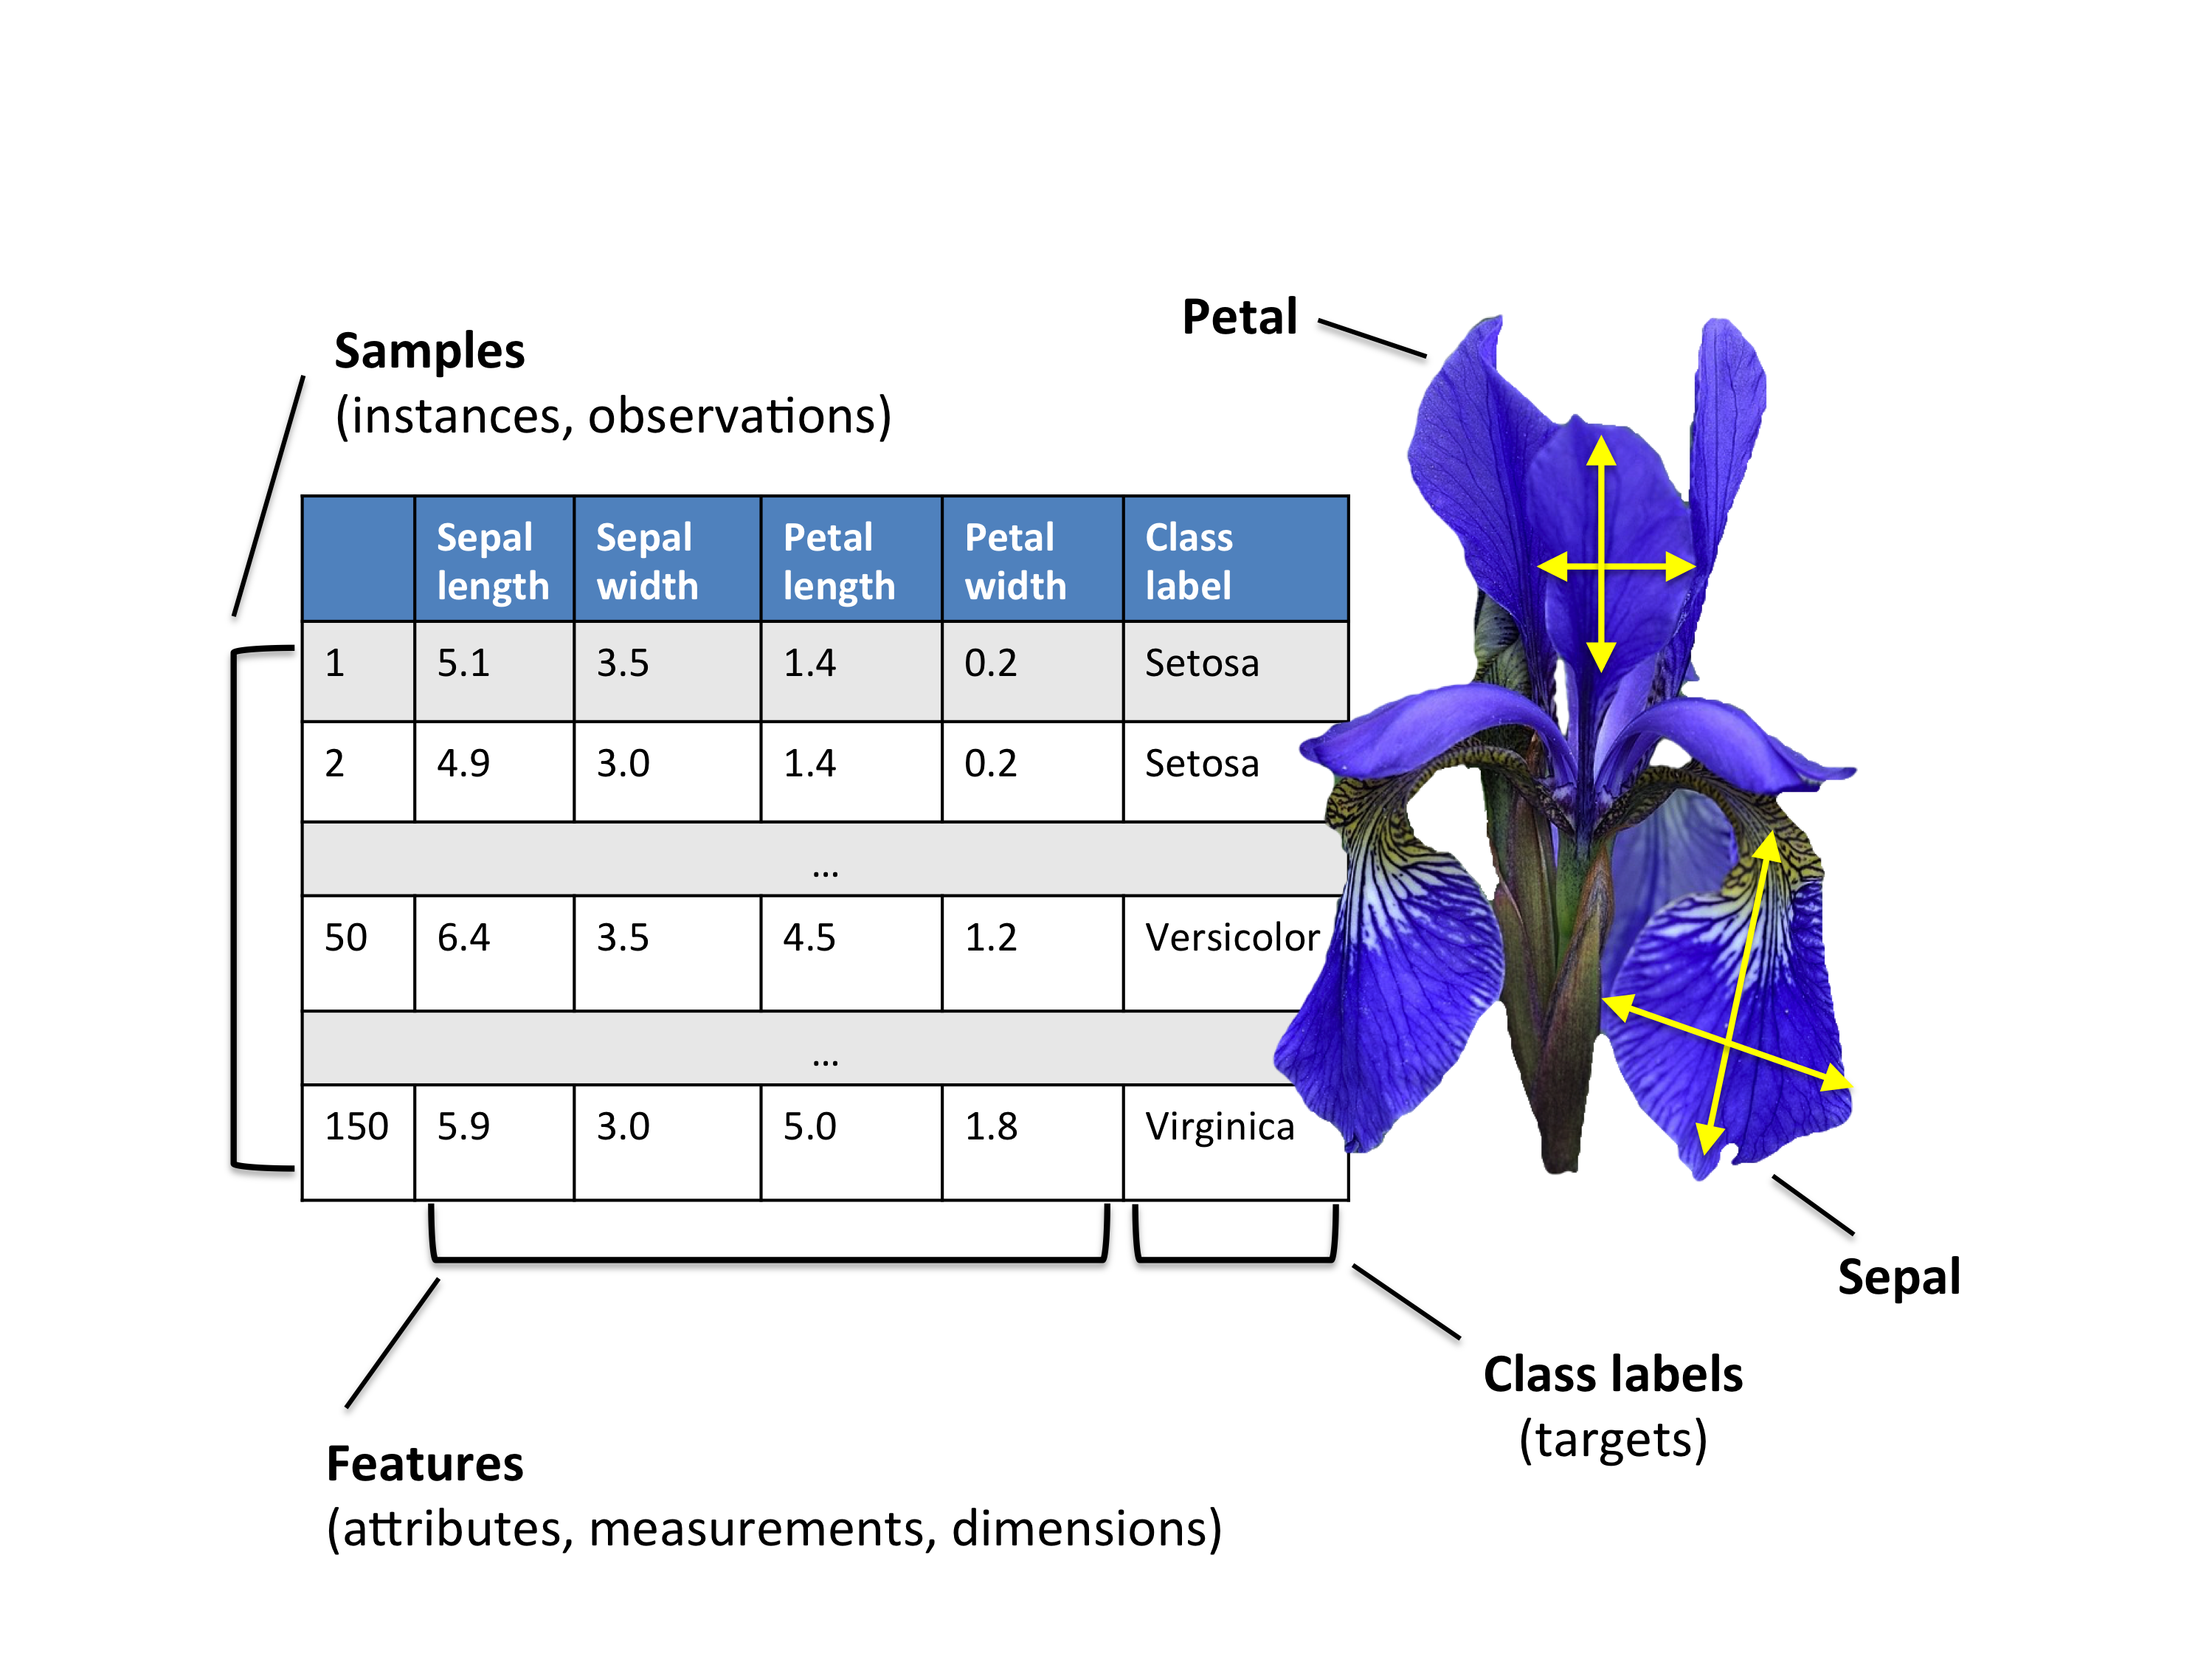
\includegraphics[scale=.1]{iris}
				\caption{Struttura dataset}
				\label{fig:iris}
			\end{center}
		\end{figure}

		

		\subsubsection{Subsubsection 3} % Sub-sub-section

			\begin{description} % Numbered list example

				\item[First] \hfill \\
				\lipsum[9] % Dummy text
				
				\item[Second] \hfill \\
				\lipsum[10] % Dummy text
				
				\item[Third] \hfill \\
				\lipsum[11] % Dummy text
			
			\end{description} 

\section{Caso di studio} % Major section

	\lipsum[12-13]
	
\newpage
\section{Codice Python completo}
	\lstinputlisting[firstline=1, lastline=59]{code/PCA.py}
	\newpage
	\lstinputlisting[firstline=61, lastline=126]{code/PCA.py}
	\newpage
	\lstinputlisting[firstline=128, lastline=174]{code/PCA.py}

%----------------------------------------------------------------------------------------
%	BIBLIOGRAPHY
%----------------------------------------------------------------------------------------

\begin{thebibliography}{99} % Bibliography - this is intentionally simple in this template

\bibitem[Figueredo and Wolf, 2009]{Figueredo:2009dg}
Figueredo, A.~J. and Wolf, P. S.~A. (2009).
\newblock Assortative pairing and life history strategy - a cross-cultural
  study.
\newblock {\em Human Nature}, 20:317--330.
 
\end{thebibliography}

%----------------------------------------------------------------------------------------

\end{document}